\section{Resultados e discussões}
\subsection{Princípio de Arquimedes}

No experimento com os pesos, foram registrados os seguintes valores ao serem colocados na jarra:

\begin{table}[H]
    \centering
    \caption{Valores dos pesos submersos}
    \begin{tabular}{|c|c|c|c|c|}
        \hline
        Massa (g) & Volume (cm$^3$) & \makecell{Massa aparente \\ pela balança
        (g)} & \makecell{Massa aparente \\ pelo dinamômetro (g)} & Afundou? \\ \hline
        688 & 702 & 692 & 0 & Não \\ \hline
        1337 & 702 & 709 & 675 & Sim \\ \hline
    \end{tabular}
\end{table}

Ao colocar o primeiro cilindro na água ele não afundou e a corda do dinamômetro relaxou, indicando que ele encontrava-se em equilíbrio vertical pelo balanço entre a força peso e o empuxo que a água fazia sobre ele, empurrando-o para cima. Para um objeto flutuar sua densidade deve ser menor que a da água (0,997g/cm\(^3\) à 25°C). É possível calcular a densidade do cilindro por:
\begin{align*}
    \frac{m} {V} = \rho
\end{align*}
\begin{align*}
    \frac{688g}{702cm^3} \cong 0,980 \mbox{g/}cm^3 < 0,997\mbox{g/}cm^3
\end{align*}
Portanto, ele era de fato menos denso que a água. Ademais, o par ação-reação do
expuxo ``empurra'' a água para baixo, de forma que o peso do cilindro era detectado pela balança (já que para o objeto estar em equilíbrio o empuxo deve igualar-se em módulo ao peso). Sendo que a detecção de 692g ao invés de 702g, uma pequena diferença, provavelmente foi acarretada de erros experimentais, que são discutidos mais adiante.

Já o segundo cilindro era mais denso que a água:
\begin{align*}
    \frac{1337g}{702cm^3} \cong 1,90 \mbox{g/cm}^3 > 0,997\mbox{g/cm}^3
\end{align*}
    
Isso resultou no fato dele afundar, como foi observado. Logo, pode-se concluir que o empuxo sobre o cilindro era inferior ao seu peso (já que para um objeto afundar as forças empurrando-o para baixo devem ser mais intensas que aquelas que o empurram para cima), tendo sido necessária a tração do dinamômetro para que o cilindro não afundasse mais, assim colocando-o em equilíbrio, como indica o diagrama de forças:

\begin{figure}[H]
    \centering
    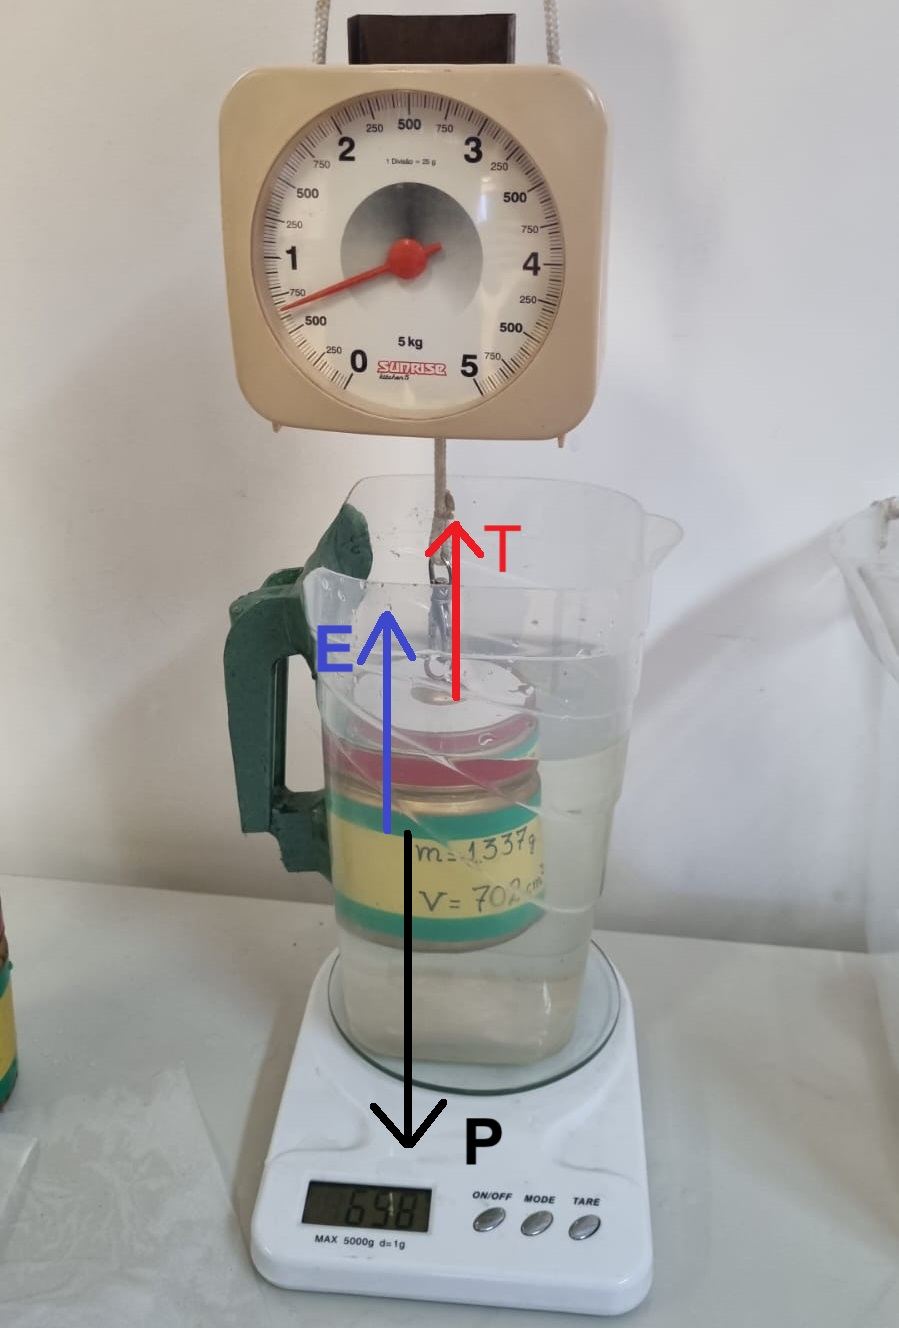
\includegraphics[width=0.4\textwidth]{fig/DiagramaDeForcas.jpeg}
    \caption{Diagrama de forças sobre segundo cilindro}
    \label{fig:diagramaForcas}
\end{figure}
Legenda do diagrama:

T: tração realiazada pelo dinamômetro;

E: empuxo;

P: força peso.
\\

Pela fórmula do expuxo (\(\mbox{E} = \mbox{V} \cdot \rho \cdot \mbox{g}\)), sendo E sua variável, e utilizando \(g = 9,7\mbox{m/s}^2\), uma vez que todo o volume do objeto estava submerso, temos:
\begin{align*}
    E = 702cm^3 \cdot 0,997g/cm^3 \cdot 9,8m/s^2
\end{align*}
\begin{align*}
 702cm^3 \cdot 0,000997kg/cm^3 \cdot 9,8m/s^2= 6,8589612 \cong 6,9 N
\end{align*}
Como o dinamômetro calcula a massa a partir do peso aparente do objeto que carrega, a tração do dinamômetro (T), convertendo-se 675g medidos em 0,675kg, pode ser calculada por:
\begin{align*}
    T = 0,675kg \cdot 9,8 m/s^2 = 6,615N \cong 6,6 N
\end{align*}
Já o peso do cilindro era:
\begin{align*}
    1337g \cdot 9,8 \mbox{m/s}^2
\end{align*}
\begin{align*}
    1,337kg \cdot 9,8 \mbox{m/s}^2 = 13,1026N \cong 13 N
\end{align*}
%Acreditam que nas contas acima seria melhor colocar os valores em algarismos significativos direto, deixar os valores com mais casas mesmo sem aproximação ou manter com as duas versões como está?
Para o sistema estar em equilíbrio, as forças deveriam se cancelar:
\begin{align*}
    E + T = P
\end{align*}
\begin{align*}
    6,9N + 6,6N = 13,5N \cong  13N 
\end{align*}
    Os valores obtidos são próximos, porém não equivalem exatamente, portanto devemos considerar causas para o erro. Considerando as incertezas envolvidas na equação \( \mbox{V} \cdot \rho \cdot \mbox{g} +md \cdot g = m \cdot g\), sendo ``md'' a massa indicada pelo dinamômetro, temos:
%Precisa justificar cada incerteza? (Tipo dizer porque de g seria 0,1)
\begin{align*}
\left( \frac{\partial }{\partial V} V \cdot \rho \cdot g \cdot \sigma V \right)^{2} = \left( \rho \cdot g \cdot \sigma V \right)^{2} =  \left( 0,977 \cdot 9,8 \cdot 0,001 \right)^{2} =A
\end{align*}
\begin{align*}
\left( \frac{\partial }{\partial g} g \cdot \rho \cdot V \cdot \sigma g \right)^{2} =  \left( \rho \cdot V \cdot \sigma g \right)^{2} = \left( 0,977 \cdot 0,702 \cdot 0,1 \right)^{2} =B
\end{align*}
\begin{align*}
\left( \frac{\partial }{\partial \rho} \rho \cdot g \cdot V \cdot \sigma \rho \right)^{2} = \left( g \cdot V \cdot \sigma \rho \right)^{2} = \left( 9,8 \cdot 0,702 \cdot 0,002 \right)^{2} =C
\end{align*}
\begin{align*}
\left( \frac{\partial }{\partial \mbox{md}} \mbox{md} \cdot g \cdot \sigma \mbox{md} \right)^{2} = \left( g \cdot \sigma \mbox{md} \right)^{2} = \left( 9,8 \cdot 0,001 \right)^{2} =D
\end{align*}
\begin{align*}
\left( \frac{\partial }{\partial g} g\cdot \mbox{md} \cdot \sigma g \right)^{2} = \left( \mbox{md} \cdot \sigma g \right)^{2} = \left( 0,675 \cdot 0,1 \right)^{2} =E
\end{align*}
\begin{align*}
\left( \frac{\partial }{\partial m} m \cdot g \cdot \sigma m \right)^{2} = \left( g \cdot \sigma m \right)^{2} = \left( 9,8 \cdot 0,001 \right)^{2} =F
\end{align*}
\begin{align*}
\left( \frac{\partial }{\partial g} g \cdot m \cdot \sigma g \right)^{2} = \left( m \cdot \sigma g \right)^{2} = \left( 1,337 \cdot 0,1 \right)^{2} =G
\end{align*}
\begin{align*}
\sqrt{A+B+C+D+E+F+G} \cong \pm 0,2
\end{align*}
Como a propagação de incerteza calculada a partir dos valores usados não é suficiente para cobrir o erro notado, espera-se que outros fatores devem ter afetado a medição, como pequenas movimentações do cilindro, o não relaxamento total do cabo do dinanômetro (de forma que ele continuasse realizando uma tração para cima), submersão de mais material além do cilindro (como o gancho e o cabo do dinamômetro) e/ou tara incorreta da balança. Tais fatores também podem ter acarretado na divergência de massa medida no primeiro cilindro, abordada anteriormente.

\subsubsection{Ouro}
Para descobrir o material que compunha o objeto denominado ``ouro'', será calculada sua densidade. Na balança obteve-se sua massa, 1150g (1,150kg) e, ao submergí-lo na jarra, porém sem deixá-lo encostar no fundo, a massa aparente ficava de 147g (0,147kg) (sendo esse valor acarretado do par ação-reação do empuxo que a água realiza sobre o objeto, como discutido anteriormente). O valor indicado pela balança é calculado a partir da força sobre ela, então:
\begin{align*}
    E = 0,147kg \cdot 9,8 \mbox{m/s}^2 = 1,4406N \cong 1,4N
\end{align*}
E temos:
\begin{align*}
    \mbox{E} = \mbox{V} \cdot \rho \cdot \mbox{g} \Rightarrow V = \frac{E}{\rho \cdot g}
\end{align*}
\begin{align*}
    V = \frac{0,147kg \cdot 9,8\mbox{m/s}}{0,977 \mbox{g/cm}^3 \cdot 9,8\mbox{m/s}^2} 
\end{align*}
\begin{align*}
    \frac{147 \mbox{g}}{0,977 \mbox{g/cm}^3} \cong 150 cm^3
\end{align*}
Assim, a densidade será:
\begin{align*}
    \frac{1150g}{150\mbox{cm}^3} \cong 7,64 \mbox{g/cm}^3
\end{align*}
Para calcular a incerteza, devemos considerar que a junção dos cálculos feitos fica: (tome \(\rho\)a como a densidade da água, m como massa e ma como massa aparente e considerando os valores em g/cm\(^3\) e g)
\begin{align*}
    \rho = \frac{m}{V} = \frac{m}{\frac{E}{\rho a \cdot g}} = \frac{m \cdot \rho a}{ma} 
\end{align*}
\begin{align*}
\left( \frac{\partial }{\partial m}m\cdot\rho a \cdot \frac{1}{ma} \cdot \sigma m \right)^2 =\left(\rho a \cdot \frac{1}{ma} \cdot \sigma m \right)^2 = \left(0,977 \cdot \frac{1}{147} \cdot 1 \right)^2 = H
\end{align*}
\begin{align*}
    \left( \frac{\partial }{\partial \rho a}m\cdot\rho a \cdot \frac{1}{ma} \cdot \sigma \rho a \right)^2 =  \left(m\cdot \frac{1}{ma} \cdot \sigma \rho a \right)^2 = \left(1150\cdot \frac{1}{147} \cdot 0,001 \right)^2 = I
\end{align*}
\begin{align*}
    \left( \frac{\partial }{\partial ma}m\cdot\rho a \cdot \frac{1}{ma} \cdot \sigma ma \right)^2  = \left(-(ma)^{-2} \cdot m\cdot\rho a \cdot \sigma ma \right)^2 \\ = \left(- (147)^{-2} \cdot 1150 \cdot 0,977 \cdot 1 \right)^2 = J
\end{align*}
\begin{align*}
    \sqrt{H + I + J} \cong \pm 0,05
\end{align*}
Ao analisar algumas tabelas de massas específicas de materiais, infere-se que o objeto pode ser feito de aço ou ferro, cuja massa específica é de aproximadamente 7,8 g/cm\(^3\).\footnote{Retirado de https://www.sucrana.com.br/tabelas/peso-especifico-materiais.pdf}\footnote{https://portal.if.usp.br/labdid/sites/portal.if.usp.br.labdid/files/densidade.pdf}
Embora sua diferença em relação ao valor calculado seja superior à incerteza prevista, foi o material mais próximo encontrado, indicando a possibilidade de terem ocorridos erros não esperados pelo cálculo de incerteza.


\subsection{Balança de empuxo}

Os dados coletados foram sintetizados na \cref{tab1} junto aos valores
disponibilizados na ficha técnica dos aparelhos.
\begin{table}[H]
    \caption{Resultados da balança de empuxo e valores de referência}
    \label{tab1}
    \begin{center}
        \begin{tabular}{c c c}
            \hline
            Item & Peso medido & Valor de referência\\
            \hline
            Peso redondo & \( (510 \pm 25) \unit{\gram} \) & \( - \) \\
            HD & \( (640 \pm 25) \unit{\gram} \) & \( - \) \\
            Celular Q. & \( (270 \pm 25) \unit{\gram} \) & \( 308 \unit{\gram} \) \\
            Celular B. & \( (250 \pm 25) \unit{\gram} \) & \( 204 \unit{\gram} \) \\
            Celular M & \( (200 \pm 25) \unit{\gram} \) & \( 169 \unit{\gram} \) \\
            Celular J. & \( (170 \pm 25) \unit{\gram} \) & \( 169 \unit{\gram} \) \\
            Celular L. & \( (220 \pm 25) \unit{\gram} \) & \( 177 \unit{\gram} \) \\
            \hline
    \end{tabular}
    \end{center}
\end{table}
As medidas obtidas variaram entre 170 g e 270 g, veja a distribuição na
\cref{pesos}, refletindo diferenças nos modelos e materiais dos aparelhos. Em
relação a diferença das massas medidas na balança com os valores de referência,
podemos atribuir esse erro a fatores como a calibração da balança, a inclinação
da garrafa em relação ao plano horizontal e, principalmente, a pesagem dos
celulares junto com suas capas protetoras.
\begin{figure}[H]
    \centering
    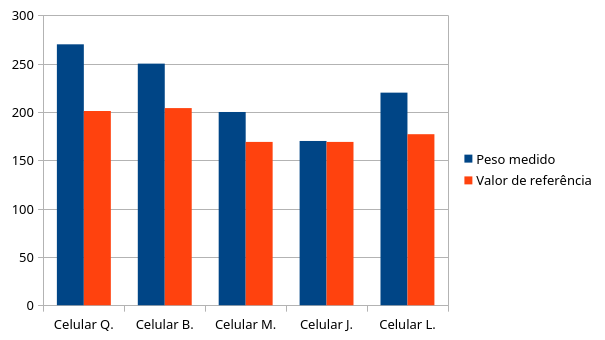
\includegraphics[width=.5\linewidth]{fig/pesos.png}
    \caption{Distribuição de peso e comparação com referência}
    \label{pesos}
\end{figure}
Note, inclusive, que o peso medido do Celular J. possui a melhor aproximação de
seu valor de referência, o que contribui com a hipótese de que o erro está
fortemente associado ao uso das capas protetoras, tendo em vista que este
aparelho foi o único pesado sem capa.

\subsection{Gangorra}

Durante o experimento foram feitos os seguintes testes:
\begin{table}[H]
    \centering
    \captionsetup{name=Quadro}
    \caption*{Quadro 1: Testes da gangorra}
    \begin{tabular}{|m{2em}|m{15em}|m{13em}|}
    \hline
        \textbf{Caso} & \textbf{Posicionamento} & \textbf{Resultado} \\ \hline
        1 & Colocar pedra na água & Gangorra tomba para seu lado \\ \hline
        2 & Colocar pedra lentamente no barco que estava sobre a água, com ambos boiando no final & Gangorra não tomba \\ \hline
        3 & Colocar pedra rapidamente no barco que estava sobre a água & Gangorra tomba para seu lado \\ \hline
        4 & Barco cheio de água (até acima do nível à sua volta) & Gangorra tomba para seu lado \\ \hline
        5 & Retirar pedra lentamente do barco & Gangorra não tomba \\ \hline
        6 & Retirar pedra rapidamente do barco & Gangorra tomba para o outro lado \\ \hline
    \end{tabular}
    \label{TabGangorra}
\end{table}
Dentre esses, serão discutidos mais a fundo o primeiro e o segundo, por responderem à questão problema do experimento.

\subsubsection{Primeiro caso: pedra sozinha}
O fato da gangorra ter caído para o lado da pedra indica que este estava mais pesado, de forma que o torque resultante fez a balança tombar para esse lado. Quando a pedra foi colocada na água ela deslocou um volume de água equivalente a seu volume, assim aumentando o nível da água. Porém, como a pedra era mais densa que a água, o peso da água do outro lado que ocupava o mesmo espaço que a pedra era inferior ao peso da pedra, como indicado na Figura \ref{figGangorra}. Assim, o maior peso da pedra resultou em uma força maior aplicada ao seu lado da balança, o que acarretou em um torque e movimento para o seu lado.
\begin{figure}[H]
    \centering
    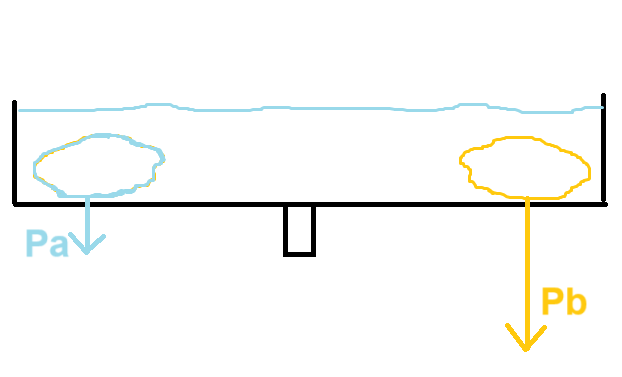
\includegraphics[width=0.5\textwidth]{fig/Gangorra.png}
    \caption{Diagrama da gangorra com pedra, logo antes de tombar}
    \label{figGangorra}
\end{figure}
Pa: peso da massa de água do outro lado que ocupava o mesmo volume que a pedra;

Pb: peso da pedra.

\subsubsection{Segundo caso: pedra no barco}
Quando a pedra foi colocada no barco lentamente ele afundou um pouco, deslocando água e assim fazendo o nível do fluído subir, porém sem tombar a gangorra. Isso significa que a massa dos dois lados permaneceu aproximadamente equivalente e realizando torques similares, ou seja, estava distribuída horizontalmente de forma homogênea. Isso aconteceu porque o peso do barco (por barco refere-se ao conjunto barco+ar dentro+pedra) foi completamente balanceado pelo empuxo (perceptível por ele não afundar). Portanto, o peso do volume de água que ele deslocou equivalia ao seu peso, como mostrado no diagrama abaixo:
\begin{figure}[H]
    \centering
    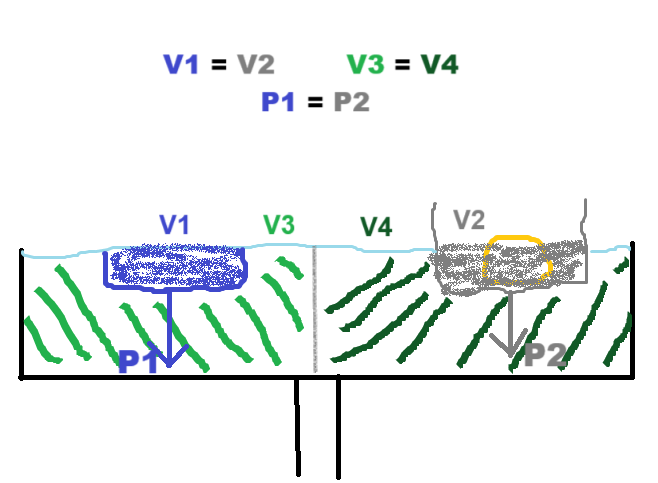
\includegraphics[width=0.5\textwidth]{fig/Gangorra2.png}
    \caption{Diagrama pedra no barco}
\end{figure}
V1: volume de água equivalente ao volume de água deslocado pelo barco;

V2: volume do barco que encontrava-se submerso;

V3: volume de água no lado esquerdo, à parte de V1;

V4: volume de água no lado direito;

P1: peso da água contida em V1;

P2: peso do barco (incluso barco, pedra e o ar contido nele).
\\

Pode-se considerar os pesos de V3 e V4 como equivalentes. Já o peso do barco era equivalente ao do volume V2 de água, pois pelo Princípio de Arquimedes o empuxo equivale ao peso do volume de fluído deslocado (neste caso igual a V2), e, neste caso, o empuxo era igual em módulo ao peso do barco, pois este estava em repouso (sem subir ou afundar).

\subsubsection{Análise dos casos 1 e 2}
A partir do raciocínio descrito, pode-se concluir que, caso um objeto permaneça flutuando (por ser, no total, menos denso que a água), ele não afetará o equilíbrio da gangorra. Isso porque o volume de água deslocado terá um peso equivalente ao do objeto, assim o outro lado que possui o volume de fluído ao invés do objeto apresentará mesmo peso e torque. Entretanto, se o objeto for mais denso que a água, a massa extra não será compensada pelo deslocamento de fluído.

\subsection{Demais casos}
No caso 4 a gangorra tombou por haver mais água no lado com o barco (que sustentava parte do líquido acima do nível da água à sua volta), assim havendo maior concentração de massa do seu lado.

O caso 5 equivale ao caso 2, embora em ordem contrária. Conforme a pedra foi retirada, o peso total do barco reduziu e ele subiu em relação ao nível da água até chegar ao equilíbrio. Como foi feito lentamente houve tempo para que a água retornasse para o lado do barco sem causar tombamento pela diferença de massas.

O caso 3 apresentou tombamento pelo acréscimo rápido da pedra fazer com que seu lado por alguns instantes pesasse consideravelmente mais que o outro, pois ainda não havia tido tempo suficiente para a água deslocar-se e igualar o nível.

De forma análoga, no caso 6 a retirada repentina da pedra faz com que seu lado pesasse menos e, antes que o barco subisse pelo retorno da água do outro lado, esse segundo por ter mais massa acabou tombando.

\subsection{Bonecos flutuantes}

Todos os integrantes do grupo foram capazes de realizar o desafio proposto, veja
a \cref{figdesafio}. Além disso, observou-se que, ao pressionar a garrafa, o
boneco submergia, retornando à posição flutuante quando a pressão era liberada.
O movimento do boneco ocorria de maneira consistente, independentemente do local
onde a garrafa era apertada, sugerindo uma relação direta com a variação de
pressão no interior do recipiente. O fenômeno se repetiu de forma idêntica em
todas as tentativas realizadas.

\begin{figure}[H]
    \centering
    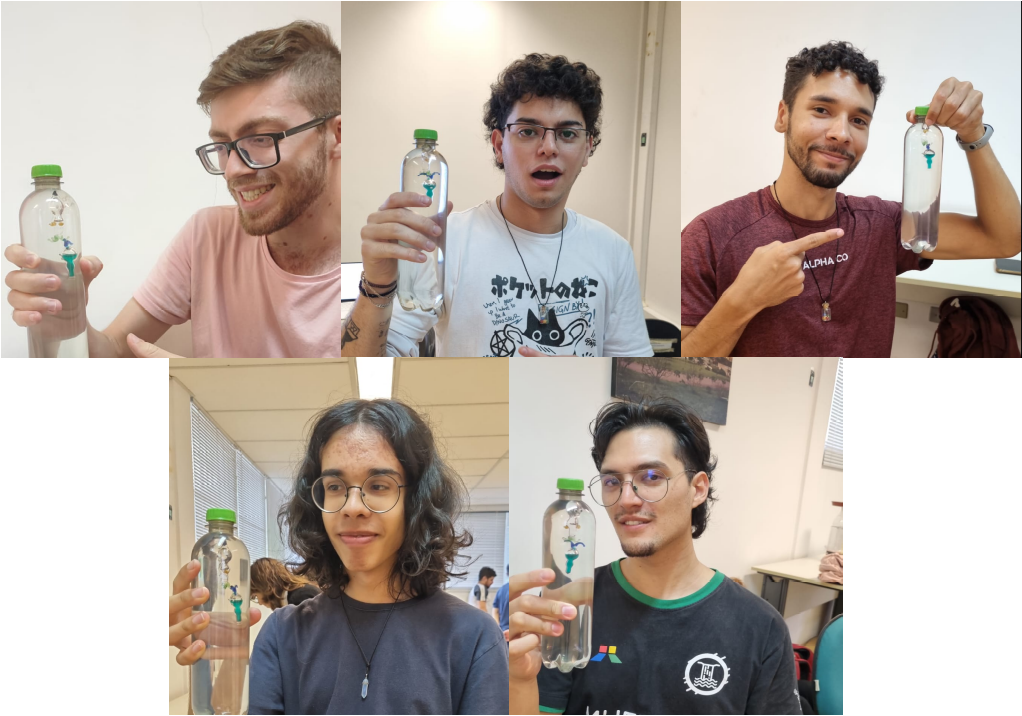
\includegraphics[width=.5\linewidth]{fig/desafio.png}
    \caption{Integrantes do grupo sorrindo após concluírem o desafio}
    \label{figdesafio}
\end{figure}

O comportamento do boneco dentro da garrafa pode ser explicado pelos princípios
da hidrostática e da variação de pressão. Já sabemos, que o boneco flutuante possui uma
cavidade com ar em sua parte inferior, o que garante sua flutuação inicial
devido ao volume deslocado de água, que gera empuxo maior que o peso do boneco.
Quando a garrafa é pressionada, a pressão hidrostática no interior do líquido
aumenta, comprimindo o ar dentro do boneco e reduzindo seu volume de água
deslocado. Consequentemente, o empuxo diminui, fazendo com que o boneco desça.
Em relação ao boneco não-flutuante, a quantidade inicial de ar em sua cavidade
é menor e, consequentemente, sua força empuxo é menor. Nesse caso, a força
empuxo é menor que a força peso e, assim, o boneco não flutua mesmo sem aumento
da pressão externa. Dessa forma, observou-se que para vencer o desafio
proposto era necessário utilizar os ganchos no boneco flutuante para segurar o
boneco não-flutuante, que foi possível pois a soma das forças de empuxo dos
bonecos era superior a soma de suas forças peso.

Além disso, quanto à posição em que a garrafa é apertada, não há diferença
aparente no movimento do boneco, dado que, de acordo com o Princípio de Pascal,
a pressão aplicada em um fluido incompressível se transmite integralmente em
todas as direções. Portanto, independentemente do local onde se pressiona a
garrafa, a variação de pressão será a mesma em todo o sistema, resultando no
mesmo efeito sobre o boneco.

